\newpage
\section{Qualità di processo}

	Per garantire la qualità del prodotto finale è necessario garantire la qualità dei processi necessari al suo completamento. A questo scopo, si è deciso di adottare lo standard \textit{ISO/IEC 15504\ped{G}}, denominato \textit{SPICE\ped{G}}.
	Esso si fonda sul principio che ogni processo deve essere controllato costantemente, in modo tale da rilevare possibili errori o debolezze, e correggerli prima che essi si diffondano, provocando un aumento del carico di lavoro e dello spreco di risorse.
	\textit{SPICE\ped{G}} definisce sei livelli di maturità del processo:
	
	\begin{itemize}
		\item \textbf{Level 0 - Incomplete:} processo non ancora implementato o incapace di raggiungere i suoi obiettivi;
		\item \textbf{Level 1 - Performed:} processo messo in atto e capace di raggiungere i suoi obiettivi;
		\item \textbf{Level 2 - Managed:} processo eseguito sulla base di obiettivi ben definiti;
		\item \textbf{Level 3 - Established:} processo eseguito in base ai principi dell’ingegneria del software; 
		\item \textbf{Level 4 - Predictable:} processo attuato all’interno di limiti ben definiti;
		\item \textbf{Level 5 - Optimizing:} processo predicibile e capace di adattarsi per raggiungere obiettivi specifici e rilevanti;
	\end{itemize}
	
	Al fine di perseguire correttamente questo modello, è necessario adottare il principio \textit{PDCA\ped{G}}, il quale si compone delle seguenti quattro fasi:
	
	\begin{itemize}
		\item \textbf{Plan:} fase di pianificazione ed individuazione di obiettivi e processi necessari allo scopo di raggiungere i risultati attesi;
		\item \textbf{Do:} fase di attuazione delle attività pianificate nella precedente fase e raccolta di dati sulla qualità ottenuta;
		\item \textbf{Check:} fase di verifica dove vengono confrontati i dati in uscita dalla fase Do con quelli pianificati nella fase Plan;
		\item \textbf{Act:} fase in cui si determinano le cause delle differenze fra risultati ottenuti e risultati attesi, in modo da individuare le azioni correttive da effettuare per ottenere un miglioramento della qualità.
	\end{itemize}

	\begin{figure}[H]
		\centering
		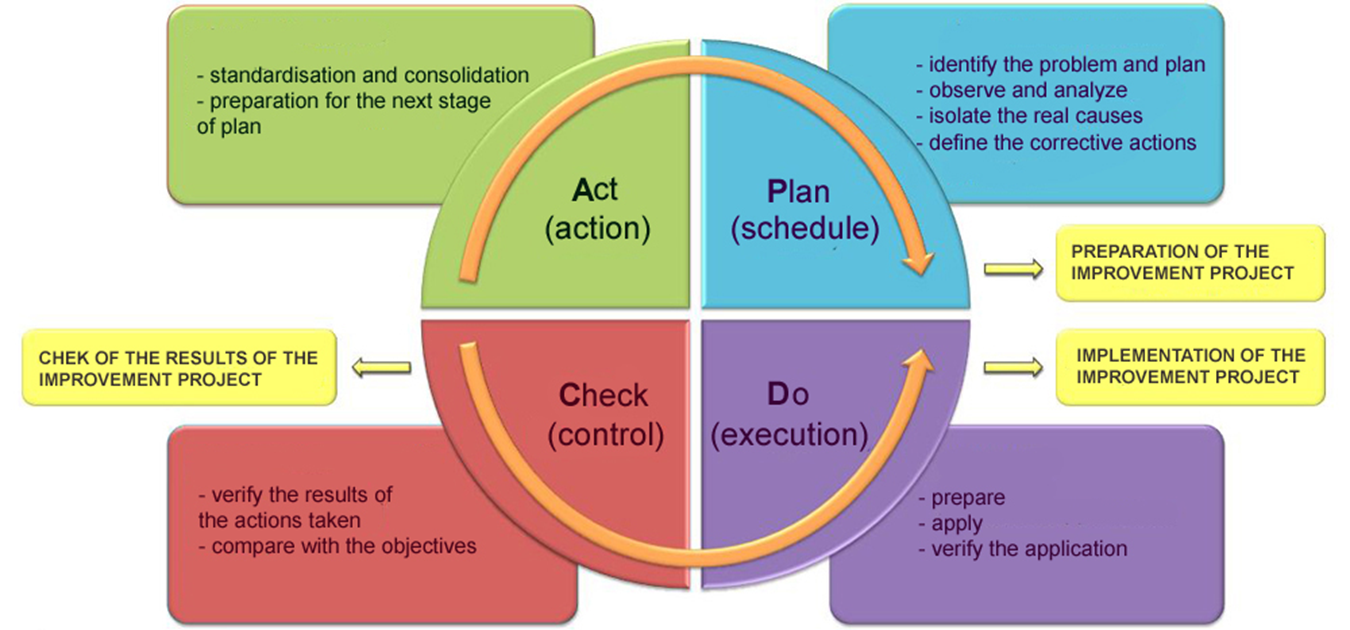
\includegraphics[scale=0.6]{includes/img/pdca.png}
		\caption{Fasi del principio PDCA.}
	\end{figure}

	Infine, il \textit{team\ped{G}} ha individuato dallo standard \textit{ISO/IEC 12207:2008\ped{G}} i processi che ritiene più importanti durante tutto il ciclo di vita del prodotto, al fine di garantire una buona qualità di processo. Per ognuno di essi sono stati individuati obiettivi e metriche coerenti con i livelli di qualità perseguiti.
	
	\subsection{Infrastructure Management Process}
	Questo processo ha lo scopo di fornire, mantenere ed aggiornare l’infrastruttura ed i servizi necessari alla realizzazione del progetto, durante tutto il suo ciclo di vita. Il termine infrastruttura comprende: elementi hardware, software, metodi, strumenti, tecniche e standard impiegati nello sviluppo del prodotto.
	Essa sarà necessaria allo svolgimento del progetto e dovrà essere mantenuta costantemente aggiornata.
	L'utilizzo delle metriche scelte, permetterà di individuare eventuali errori all’interno degli strumenti utilizzati, la cui correzione permetterà di produrre dati corretti e coerenti.
		\subsubsection{Obiettivi}
		Per tutta la durata del progetto, l’infrastruttura impiegata nello sviluppo dovrà raggiungere i seguenti obiettivi:
		\begin{itemize}
			\item ogni procedura riguardante le attività svolte più frequentemente durante lo sviluppo del
			progetto, sarà descritta nel documento \textsc{NormeDiProgetto 1\_0\_0.pdf};
			\item ogni riferimento normativo ed informativo sarà completo di informazioni utili al proprio
			reperimento;
			\item la piattaforma \textit{NetBreakDB} sarà a disposizione di ogni componente del team, in caso di bisogno di accesso ai dati in essa contenuti;
		\end{itemize}
		\subsubsection{Metriche}
			\paragraph{Disponibilità NetBreakDB}
			Indica la percentuale di disponibilità di utilizzo della piattaforma NetBreakDB, rispetto alle richieste di accesso.
			
			\begin{itemize}
				\item \textbf{nacclogin} = numero accessi corretti alla pagina di login
				\item \textbf{naclogintot} = totale delle richieste di accesso alla pagina di login inoltrate
				\item \textbf{disp} = \begin{math}
				\frac{nacclogin}{naclogintot}
				\end{math} 
			\end{itemize}
			
			\begin{table}[H]
				\begin{longtable}{>{\centering\arraybackslash}p{5cm}|>{\centering\arraybackslash}p{5cm} | >{\centering\arraybackslash}p{5cm}}
					\hline
					\rowcolor{Gray}
					\textbf{Metodo di calcolo} & \textbf{Range accettazione} & \textbf{Range ottimale} \\
					\hline
					disp & [80,100] in [0,100]  & 100 in [0,100] 
				\end{longtable}
				\caption{Disponibilità NetBreakDB}
			\end{table}
			
			
	
	\subsection{Project Planning, Assessment \& Control Process}
	Questo processo ha lo scopo di produrre dei piani di sviluppo per il progetto, che comprendano:
	\begin{itemize}
		\item la scelta del modello di ciclo di vita del prodotto;
		\item le descrizioni delle attività e dei compiti da svolgere;
		\item la pianificazione temporale del lavoro e dei costi da sostenere;
		\item l'allocazione di compiti e responsabilità;
		\item le misurazioni per rilevare lo stato del progetto, rispetto alle pianificazioni stilate.
	\end{itemize}
	Durante tutta l’attività di	progetto, sarà fondamentale mantenere aggiornata la pianificazione effettuata, in modo da essere sempre coerente con la situazione attuale. Nel caso in cui, in una fase di lavoro, venissero rilevati dei valori negativi, attraverso l'utilizzo delle metriche scelte Schedule Variance e Budget Variance, occorrerà compensare tali valori entro la fine dell’attività di progetto, al fine di evitare di eccedere le ore di lavoro totali e, di conseguenza, il preventivo dei costi finale indicato nella pianificazione contenuta nel documento \textsc{PianoDiProgetto 1\_0\_0.pdf}.
		\subsubsection{Obiettivi}
		L’intero sviluppo del progetto dovrà seguire la pianificazione prodotta:
		\begin{itemize}
			\item ogni componente dovrà svolgere e portare a termine l'attività assegnatagli, svolgendo tutti i compiti nei quali è stata suddivisa e facendo attenzione a rispettare le scadenze fissate;
			\item il costo necessario allo svolgimento di un'attività non dovrà eccedere la somma
			preventivata.
		\end{itemize}
		\subsubsection{Metriche}
			\paragraph{Schedule Variance}
			Indica se si è o meno in linea con la pianificazione temporale delle attività nella baseline.
			Se si ottiene 0 significa che il team ha rispettato la pianificazione, altrimenti significa che è in ritardo.
			
				\begin{itemize}
				\item \textbf{attcompl} = attività effettivamente completate
				\item \textbf{atttot} = attività totali in linea con la pianificazione
				\item \textbf{schedulevar} = \begin{math}
				\frac{atttot - attcompl}{atttot}
				\end{math} 
			\end{itemize}
			
			\begin{table}[H]
				\begin{longtable}{>{\centering\arraybackslash}p{5cm}|>{\centering\arraybackslash}p{5cm} | >{\centering\arraybackslash}p{5cm}}
					\hline
					\rowcolor{Gray}
					\textbf{Metodo di calcolo} & \textbf{Range accettazione} & \textbf{Range ottimale} \\
					\hline
					schedulevar & schedulevar <= 0.2 in [0,1]  & schedulevar <= 0.1 in [0,1] 
				\end{longtable}
				\caption{Schedule Variance}
			\end{table}
			

		
		\paragraph{Budget Variance}
		Indica se la spesa sostenuta alla data corrente è superiore o inferiore a quella preventivata in sede di pianificazione.
		Un valore positivo indica che si è speso meno di quanto inizialmente previsto, altrimenti significa che si è speso più del preventivo.
		
		\begin{itemize}
			\item \textbf{costopiano} = costo pianificazione per realizzare attivit\`{a} di progetto alla data corrente
			\item \textbf{costotot} = spesa effettiva alla data corrente
			\item \textbf{budgetvar} = costopiano - costotot
		\end{itemize}
		
		\begin{table}[H]
			\begin{longtable}{>{\centering\arraybackslash}p{5cm}|>{\centering\arraybackslash}p{5cm} | >{\centering\arraybackslash}p{5cm}}
				\hline
				\rowcolor{Gray}
				\textbf{Metodo di calcolo} & \textbf{Range accettazione} & \textbf{Range ottimale} \\
				\hline
				budgetvar & schedulevar >= 0 in [0,100]  & 100 in [0,100] 
			\end{longtable}
			\caption{Budget Variance}
		\end{table}
		
	
	\subsection{Risk Management Process}
	Questo processo ha l'obiettivo di identificare, analizzare, trattare e monitorare in modo continuo i rischi che possono insorgere durante l’intera attività di progetto.
	Il livello di probabilità dei rischi analizzati dovrà essere costantemente monitorato. Nel caso si manifestasse un rischio, a qualsiasi livello di pericolosità, il team dovrà attuare le contromisure previste, al fine di mitigare i suoi effetti ed evitare un incremento del livello di pericolosità.
		\subsubsection{Obiettivi}
		Il team dovrà gestire correttamente i rischi:
		\begin{itemize}
			\item all’inizio dell’attività di progetto, verranno individuati i principali fattori di rischio riguardanti l’organizzazione delle attività;
			\item all’inizio di ogni attività, l’analisi dei rischi potrà portare all’individuazione di nuovi specifici rischi per ognuna di esse;
			\item i rischi analizzati che si manifesteranno, verranno trattati secondo le strategie descritte, così da controllarne l'impatto.
		\end{itemize}
		\subsubsection{Metriche}
			\paragraph{Rischi non preventivati}
			Indicatore che evidenzia i rischi non preventivati.
			
			\begin{itemize}
				\item \textbf{rischinoninar} = un contatore registra i rischi non identificati in analisi dei requisiti
			\end{itemize}
			
			\begin{table}[H]
				\begin{longtable}{>{\centering\arraybackslash}p{5cm}|>{\centering\arraybackslash}p{5cm} | >{\centering\arraybackslash}p{5cm}}
					\hline
					\rowcolor{Gray}
					\textbf{Metodo di calcolo} & \textbf{Range accettazione} & \textbf{Range ottimale} \\
					\hline
					rischinoninar & [0,5]  & 0 
				\end{longtable}
				\caption{Rischi non preventivati}
			\end{table}
			
			
	
	\subsection{System/Software Requirements Analysis Process}
	Questo processo ha lo scopo di creare un insieme di requisiti tecnici, a partire dall'insieme di requisiti individuati dalle fonti, in modo che diventi la linea guida nella progettazione del prodotto.
	Ogni requisito individuato dovrà essere inserito correttamente nella piattaforma NetBreakDB, la quale si occuperà di effettuare il tracciamento delle fonti dalle quali derivano i requisiti, delle modifiche effettuate e della loro implementazione nel prodotto.
		\subsubsection{Obiettivi}
		I requisiti identificati dovranno essere gestiti in modo da raggiungere i seguenti obiettivi:
		\begin{itemize}
			\item per ogni requisito dovrà essere possibile indicare dei test, da effettuare per verificarne il soddisfacimento da parte del prodotto;
			\item nessun requisito dovrà risultare ambiguo;
			\item tutti i requisiti che il prodotto andrà a soddisfare, saranno stati precedentemente approvati dai committenti.
		\end{itemize}
		\subsubsection{Metriche}
			\paragraph{Adempimento requisiti obbligatori}
			Indica la percentuale di requisiti obbligatori soddisfatti dal prodotto.
			
			\begin{itemize}
				\item \textbf{nreqobblsodd} = numero requisiti obbligatori soddisfatti
				\item \textbf{nreqobblid} = numero requisiti obbligatori identificati
				\item \textbf{adempimento} =  \begin{math}
				\frac{nreqobblsodd}{nreqobblid}
				\end{math} 
			\end{itemize}
			
			\begin{table}[H]
				\begin{longtable}{>{\centering\arraybackslash}p{5cm}|>{\centering\arraybackslash}p{5cm} | >{\centering\arraybackslash}p{5cm}}
					\hline
					\rowcolor{Gray}
					\textbf{Metodo di calcolo} & \textbf{Range accettazione} & \textbf{Range ottimale} \\
					\hline
					adempimento & [90,100] in [0,100]  & 100 in [0,100]
				\end{longtable}
				\caption{Adempimento requisiti obbligatori}
			\end{table}
			
	
	\subsection{System/Software Architectural Design Process}
	Il processo si pone come obiettivo quello di identificare una corrispondenza fra requisiti di sistema ed elementi del sistema. Nel corso dell’attività di progettazione, sia ad alto livello che di dettaglio, le componenti verranno inserite nella piattaforma NetBreakDB. Essa si occuperà di effettuare i tracciamenti fra le componenti e i requisiti che soddisfano, ed inoltre, il tracciamento tra le relazioni presenti e le varie componenti.
		\subsubsection{Obiettivi}
		Durante lo svolgimento delle attività previste da questo processo, il team punterà a definire
		un’architettura adatta agli scopi del progetto:
		\begin{itemize}
			\item ogni componente progettato come parte del sistema risulterà essere necessario per il funzionamento del prodotto e, quindi, costantemente tracciabile ai requisiti che soddisfa;
			\item il sistema dovrà presentare basso accoppiamento ed alta coesione;
			\item ogni componente dovrà essere progettato puntando su incapsulamento, modularizzazione
			e riuso di codice.
		\end{itemize}
		
		\subsubsection{Metriche}
			\paragraph{Fan In}
			In riferimento ad un modulo software, misura quanti altri moduli lo utilizzano durante la loro esecuzione.
			Tale indicazione consente di stabilire il livello di riuso implementato.
			
			\begin{itemize}
				\item \textbf{increm} = ncrementato contatore quandod viene in un oggetto viene richiamato un modulo
			\end{itemize}
			
			\begin{table}[H]
				\begin{longtable}{>{\centering\arraybackslash}p{5cm}|>{\centering\arraybackslash}p{5cm} | >{\centering\arraybackslash}p{5cm}}
					\hline
					\rowcolor{Gray}
					\textbf{Metodo di calcolo} & \textbf{Range accettazione} & \textbf{Range ottimale} \\
					\hline
					increm & increm >=0  & increm >= 3
				\end{longtable}
				\caption{Fan In}
			\end{table}
			
		
			
			\paragraph{Fan Out}
			In riferimento ad un modulo software, misura quanti moduli vengono utilizzati durante la
			sua esecuzione.
			Tale indicazione consente di stabilire il livello di accoppiamento implementato.
			
			\begin{itemize}
				\item \textbf{increm} = incrementato contatore quando individuato modulo

		\end{itemize}
	
		\begin{table}[H]
		\begin{longtable}{>{\centering\arraybackslash}p{5cm}|>{\centering\arraybackslash}p{5cm} | >{\centering\arraybackslash}p{5cm}}
			\hline
			\rowcolor{Gray}
			\textbf{Metodo di calcolo} & \textbf{Range accettazione} & \textbf{Range ottimale} \\
			\hline
			increm & [0,5] & [0,1]
		\end{longtable}
		\caption{Fan Out}
		\end{table}

			
	
	\subsection{Software Architectural Design Process}
	Lo scopo del processo è fornire una progettazione di minimo del prodotto che andrà a soddisfare i requisiti individuati.
	Tutte le attività presenti in questo processo portano alla produzione del documento Specifica Tecnica.
		\subsubsection{Obiettivi}
			\begin{itemize}
				\item fornire un'architettura ad alto livello del prodotto software, in grado di soddisfare i requisiti individuati;
				\item definire le interfacce interne ed esterne per ogni componente individuato;
				\item progettare uno schema ad alto livello del database. 
			\end{itemize}
	
	\subsection{Software Detailed Design Process}
	Lo scopo del processo è fornire una progettazione dettagliata del prodotto che andrà ad implementare i requisiti individuati.
	Sarà necessario effettuare un’analisi dettagliata delle componenti individuate durante l'attività di progettazione
	architetturale, suddividendole in unità che siano facilmente codificabili e testabili.
		\subsubsection{Obiettivi}
		Le attività svolte dovranno raggiungere i seguenti obiettivi:
		\begin{itemize}
			\item il livello di dettaglio della progettazione dovrà indicare tutti i metodi, con i relativi parametri e campi dati, forniti da ciascuna classe;
			\item la struttura a basso livello dell’architettura e le relazioni fra le varie unità software concepite saranno esposte nel documento di Definizione di Prodotto, il quale definirà esattamente cosa implementare;
		\end{itemize}
		
		\subsubsection{Metriche}
			\paragraph{Numero di metodi per classe}
			Indica il numero di metodi definiti in una classe.
			Un valore molto alto potrebbe indicare una
			non buona decomposizione delle funzionalità a livello logico.
			
			\begin{itemize}
				\item \textbf{nmetodi} = viene implementato in netbreakdb un modo per tenere traccia dei metodi di una classe e da qui \`{e} possibile estrarne il numero
			\end{itemize}
			
			\begin{table}[H]
				\begin{longtable}{>{\centering\arraybackslash}p{5cm}|>{\centering\arraybackslash}p{5cm} | >{\centering\arraybackslash}p{5cm}}
					\hline
					\rowcolor{Gray}
					\textbf{Metodo di calcolo} & \textbf{Range accettazione} & \textbf{Range ottimale} \\
					\hline
					nmetodi & [1,10] & [1,5]
				\end{longtable}
				\caption{Numero di metodi per classe}
			\end{table}
			
		
			\paragraph{Numero di parametri per metodo}
			Indica il numero di parametri passati ad un metodo.
			Un valore molto alto potrebbe indicare un'eccessiva complessità del metodo, il quale potrebbe non essere sufficientemente scomposto in sotto-metodi.
			
			\begin{itemize}
				\item \textbf{nparametri} = viene implementato in netbreakdb un modo per tenere traccia del numero dei parametri dei metodi di una classe e da qui \`{e} possibile estrarne il numero
			\end{itemize}
			
			\begin{table}[H]
				\begin{longtable}{>{\centering\arraybackslash}p{5cm}|>{\centering\arraybackslash}p{5cm} | >{\centering\arraybackslash}p{5cm}}
					\hline
					\rowcolor{Gray}
					\textbf{Metodo di calcolo} & \textbf{Range accettazione} & \textbf{Range ottimale} \\
					\hline
					nparametri & [0,8] & [0,4]
				\end{longtable}
				\caption{Numero parametri per metodo}
			\end{table}
			
		
		
			\paragraph{Numero di attributi per classe}
			Indica il numero di attributi di una classe.
			Un valore molto alto potrebbe suggerire la necessità di suddividere tale classe in più classi differenti correlate tra loro.
			
			\begin{itemize}
				\item \textbf{nattributi} = viene implementato in netbreakdb un modo per tenere traccia del numero di attributi di una classe e da qui \`{e} possibile estrarne il numero
			\end{itemize}
			
			\begin{table}[H]
				\begin{longtable}{>{\centering\arraybackslash}p{5cm}|>{\centering\arraybackslash}p{5cm} | >{\centering\arraybackslash}p{5cm}}
					\hline
					\rowcolor{Gray}
					\textbf{Metodo di calcolo} & \textbf{Range accettazione} & \textbf{Range ottimale} \\
					\hline
					nattributi & [0,12] & [2,8]
				\end{longtable}
				\caption{Numero di attributi per classe}
			\end{table}
			
			
	\subsection{Software Construction Process}
	Questo processo definisce le principali attività volte alla produzione di unità software eseguibili, che
	rispettino quanto prodotto durante la progettazione.
	Nell’attività di codifica, il \textit{\Progr} dovrà semplicemente attenersi a quanto indicato nel documento Definizione di Prodotto. Inoltre, sarà necessario procedere con la codifica dei test individuati in sede di progettazione, al fine di verificare il corretto funzionamento delle varie unità prodotte.
		
		\subsubsection{Obiettivi}
		Affinchè le unità software prodotte risultino di qualità, il team ha individuato i seguenti obiettivi:
		\begin{itemize}
			\item l’implementazione delle classi e dei metodi definiti in progettazione dovrà produrre codice a bassa complessità, in modo da facilitare l'attività di test;
			\item l’uso di costrutti e tecniche che creano sdoppiamenti del flusso di esecuzione verrà attuato solo se strettamente necessario;
			\item il codice prodotto dovrà risultare facilmente manutenibile;
			\item il codice prodotto risulterà privo di elementi inutilizzati.
		\end{itemize}
		
		\subsubsection{Metriche}
			\paragraph{Complessità Ciclomatica}
			Indica la complessità di funzioni, moduli, metodi o classi di un programma, misurando il numero
			di cammini linearmente indipendenti attraverso il grafo di controllo di flusso.
			Alti valori di complessità ciclomatica implicano una ridotta manutenibilità del codice; viceversa, bassi valori potrebbero determinare una scarsa efficienza dei metodi.
			
				\begin{itemize}
				\item \textbf{ciclomcompless} = n° archi - n° nodi + 2 
			\end{itemize}
			
			\begin{table}[H]
				\begin{longtable}{>{\centering\arraybackslash}p{5cm}|>{\centering\arraybackslash}p{5cm} | >{\centering\arraybackslash}p{5cm}}
					\hline
					\rowcolor{Gray}
					\textbf{Metodo di calcolo} & \textbf{Range accettazione} & \textbf{Range ottimale} \\
					\hline
					ciclomcompless & [0,10] & [3,10]
				\end{longtable}
				\caption{Complessità Ciclomatica}
			\end{table}
			
			
			\paragraph{Numero di livelli di annidamento}
			Indica il numero di funzioni o procedure chiamate all’interno di un metodo.
			Un valore elevato implica un’alta complessità ed un basso livello di astrazione del codice.
			
			\begin{itemize}
				\item \textbf{increm} = variabile che incrementa a ogni chiamata a funzioni da un certo metodo
			\end{itemize}
			
			\begin{table}[H]
				\begin{longtable}{>{\centering\arraybackslash}p{5cm}|>{\centering\arraybackslash}p{5cm} | >{\centering\arraybackslash}p{5cm}}
					\hline
					\rowcolor{Gray}
					\textbf{Metodo di calcolo} & \textbf{Range accettazione} & \textbf{Range ottimale} \\
					\hline
					increm & [1,8] & [1,4]
				\end{longtable}
				\caption{Numero di livelli di annidamento}
			\end{table}
			
	
		
			\paragraph{Linee di commento}
			Indica la percentuale di linee di commento presenti all’interno del codice sorgente; la loro presenza
			permette una più semplice comprensione ed un maggior livello di manutenibilità di quanto
			prodotto.
			
			\begin{itemize}
				\item \textbf{nlineecomm} = numero linee di commento presenti nel codice
				\item \textbf{sloc} = sloc totali prodotte
				\item \textbf{percentcomme} =  \begin{math}
				\frac{nlineecomm}{sloc}
				\end{math} 
			\end{itemize}
			
			\begin{table}[H]
				\begin{longtable}{>{\centering\arraybackslash}p{5cm}|>{\centering\arraybackslash}p{5cm} | >{\centering\arraybackslash}p{5cm}}
					\hline
					\rowcolor{Gray}
					\textbf{Metodo di calcolo} & \textbf{Range accettazione} & \textbf{Range ottimale} \\
					\hline
					percentcomme & [20,100] in [0, 100] & [35,100] in [0,100]
				\end{longtable}
				\caption{Linee di commento}
			\end{table}
			
		
	
	\subsection{System/Software Qualification Testing Process}
	Lo scopo del processo è quello di assicurare che ogni requisito individuato sia stato implementato nel prodotto.
	Sarà indispensabile rendere il più possibile automatizzata l’esecuzione dei test di sistema, in modo tale che la loro esecuzione non richieda costi e tempi eccessivi, e  allo stesso tempo sia possibile eseguirne un numero sufficiente a garantire un’ottima copertura
	dei requisiti.
		
		\subsubsection{Obiettivi}
		Durante lo svolgimento delle attività di test, il team dovrà perseguire i seguenti obiettivi:
			\begin{itemize}
				\item le attività di test previste dal processo verranno svolte su un sistema le cui componenti sono verificate e correttamente integrate fra loro;
				\item il sistema dovrà implementare e soddisfare tutti i requisiti obbligatori individuati durante l'attività di analisi dei requisiti.
			\end{itemize}
		
		\subsubsection{Metriche}
			\paragraph{Test di Unità}
			Indica la percentuale di test di unità eseguiti.
			
			\begin{itemize}
				\item \textbf{ntues} = numero Test Unità eseguiti
				\item \textbf{ntupian} = numero Test Unità panificati
				\item \textbf{testu} =  \begin{math}
				\frac{ntues}{ntupian}
				\end{math} 
			\end{itemize}
			
			\begin{table}[H]
				\begin{longtable}{>{\centering\arraybackslash}p{5cm}|>{\centering\arraybackslash}p{5cm} | >{\centering\arraybackslash}p{5cm}}
					\hline
					\rowcolor{Gray}
					\textbf{Metodo di calcolo} & \textbf{Range accettazione} & \textbf{Range ottimale} \\
					\hline
					testu & [95,100] in [0, 100] & 100 in [0,100]
				\end{longtable}
				\caption{Test di Unità}
			\end{table}
		
			
			\paragraph{Test di Integrazione}
			Indica la percentuale di test di integrazione eseguiti.
			
			\begin{itemize}
				\item \textbf{nties} = numero Test Integrazione eseguiti
				\item \textbf{ntipian} = numero Test Integrazione panificati
				\item \textbf{testi} =  \begin{math}
				\frac{nties}{ntipian}
				\end{math} 
			\end{itemize}
			
			\begin{table}[H]
				\begin{longtable}{>{\centering\arraybackslash}p{5cm}|>{\centering\arraybackslash}p{5cm} | >{\centering\arraybackslash}p{5cm}}
					\hline
					\rowcolor{Gray}
					\textbf{Metodo di calcolo} & \textbf{Range accettazione} & \textbf{Range ottimale} \\
					\hline
					testi & [65,100] in [0, 100] & [75, 100] in [0,100]
				\end{longtable}
				\caption{Test di Integrazione}
			\end{table}
			
			
			\paragraph{Test di Sistema}
			Indica la percentuale di test di sistema eseguiti.
			
			\begin{itemize}
				\item \textbf{ntses} = numero Test Sistema eseguiti
				\item \textbf{ntspian} = numero Test Sistema panificati
				\item \textbf{tests} =  \begin{math}
				\frac{ntses}{ntspian}
				\end{math} 
			\end{itemize}
			
			\begin{table}[H]
				\begin{longtable}{>{\centering\arraybackslash}p{5cm}|>{\centering\arraybackslash}p{5cm} | >{\centering\arraybackslash}p{5cm}}
					\hline
					\rowcolor{Gray}
					\textbf{Metodo di calcolo} & \textbf{Range accettazione} & \textbf{Range ottimale} \\
					\hline
					testi & [75,100] in [0, 100] & [85, 100] in [0,100]
				\end{longtable}
				\caption{Test di Sistema}
			\end{table}
			
			
			\paragraph{Test superati}
			Indica la percentuale di test totali superati.
			
			\begin{itemize}
				\item \textbf{ntestsup} = numero Test superati
				\item \textbf{ntesteseg} = numero Test eseguiti
				\item \textbf{testsuper} =  \begin{math}
				\frac{ntestsup}{ntesteseg}
				\end{math} 
			\end{itemize}
			
			\begin{table}[H]
				\begin{longtable}{>{\centering\arraybackslash}p{5cm}|>{\centering\arraybackslash}p{5cm} | >{\centering\arraybackslash}p{5cm}}
					\hline
					\rowcolor{Gray}
					\textbf{Metodo di calcolo} & \textbf{Range accettazione} & \textbf{Range ottimale} \\
					\hline
					testsuper & [95,100] in [0, 100] & 100 in [0,100]
				\end{longtable}
				\caption{Test di Validazione}
			\end{table}
			
			
			

	
	\subsection{Software Documentation Management Process}
	Questo processo ha l'obiettivo di produrre e manutenere le informazioni sul software prodotte dai processi
	attuati, attraverso un'opportuna documentazione.
	Ogni documento sarà dotato di:
		\begin{itemize}
			\item numero di versione;
			\item changelog.
		\end{itemize}
	Queste informazioni consentono di tenere traccia di ogni azione effettuata sul documento in oggetto.
		
		\subsubsection{Obiettivi}
		Il processo di documentazione dovrà perseguire le seguenti direttive:
			\begin{itemize}
				\item la documentazione prodotta dovrà essere chiara e comprensibile a tutti gli stakeholderG e
				sarà resa disponibile alle parti interessate per la consultazione;
				\item ogni forma di ambiguità sul significato di un termine utilizzato verrà eliminata grazie al
				Glossario;
				\item la documentazione prodotta sarà sempre aggiornata ed allineata allo stato attuale del
				processo di sviluppo del prodotto.
			\end{itemize}
		
		\subsubsection{Metriche}
			\paragraph{Indice Gulpease}
			L'indice Gulpease è un indice di leggibilità di un testo tarato sulla lingua italiana.
			Rispetto ad altri indici, questo ha il vantaggio di utilizzare la lunghezza delle parole in lettere, anziché in sillabe, semplificandone il calcolo automatico. L'indice Gulpease considera due variabili linguistiche:
			\begin{itemize}
				\item la lunghezza della parola;
				\item la lunghezza della frase, rispetto al numero delle lettere.
			\end{itemize}
			I risultati sono compresi tra 0 e 100, dove il valore 100 indica la leggibilità più alta, mentre il valore 0 la leggibilità più bassa.
			
			
			\begin{itemize}
				\item \textbf{gulpease} = 89+ \begin{math}
				\frac{300*num frasi-10*num lett}{num par}
				\end{math}
				
			\end{itemize}
			
			\begin{table}[H]
				\begin{longtable}{>{\centering\arraybackslash}p{5cm}|>{\centering\arraybackslash}p{5cm} | >{\centering\arraybackslash}p{5cm}}
					\hline
					\rowcolor{Gray}
					\textbf{Metodo di calcolo} & \textbf{Range accettazione} & \textbf{Range ottimale} \\
					\hline
					gulpease & [40,100] in [0, 100] & 100 in [0,100]
				\end{longtable}
				\caption{Indice Gulpease}
			\end{table}
			
	
	\subsection{Software Verification Process}
	Questo processo ha lo scopo di verificare se un qualsiasi elemento del sistema soddisfa in modo esaustivo i requisiti ad esso associati.
	Durante le varie attività di revisione della documentazione, gli errori più frequenti rilevati verranno
	riportati in un documento apposito, in modo tale da velocizzare le successive attività di inspection.
	Inoltre, per ogni test effettuato verrà tenuto il tracciamento del suo esito.
		
		\subsubsection{Obiettivi}
		
		
		\subsubsection{Metriche}
			\paragraph{Code Coverage}
			Indica la percentuale di istruzioni che sono eseguite durante i test.
			Un alto valore di questo indice implica un'alta probabilità che le componenti testate abbiano una ridotta quantità di errori.
			Per ottenere un indice basso è necessario che l'implementazione dei metodi sia molto semplice, in modo da non richiedere alcuna attività di testing. Ad esempio, i metodi getter e setter.
			
			\begin{itemize}
				\item \textbf{lineemonitor} = numero linee codice monitorato da test
				\item \textbf{lineeimplem} = numero linee codice implementato in sw
				\item \textbf{coverage} = \begin{math}
				\frac{lineemonitor}{lineeimplem}
				\end{math}
				
			\end{itemize}
			
			\begin{table}[H]
				\begin{longtable}{>{\centering\arraybackslash}p{5cm}|>{\centering\arraybackslash}p{5cm} | >{\centering\arraybackslash}p{5cm}}
					\hline
					\rowcolor{Gray}
					\textbf{Metodo di calcolo} & \textbf{Range accettazione} & \textbf{Range ottimale} \\
					\hline
					gulpease & [80,100] in [0, 100] & 100 in [0,100]
				\end{longtable}
				\caption{Code Coverage}
			\end{table}
			
	